\documentclass[8pt]{beamer}


%Russian-specific packages
%--------------------------------------
\usepackage[T2A]{fontenc}
\usepackage[utf8]{inputenc}
\usepackage[russian]{babel}
%--------------------------------------

\usepackage{listings}
%code
\def\code#1{\texttt{#1}}
% Зачёркивание текста
\usepackage{cancel}
% Две картинки рядом
\usepackage{subfigure}
% Нумерация страниц
\addtobeamertemplate{navigation symbols}{}{%
    \usebeamerfont{footline}%
    \usebeamercolor[fg]{footline}%
    \hspace{1em}%
    \insertframenumber/\inserttotalframenumber
}

\hypersetup{
    colorlinks=true,
    linkcolor=blue,
    filecolor=magenta,      
    urlcolor=blue,
    pdftitle={Sharelatex Example},
    bookmarks=true,
    pdfpagemode=FullScreen,
}

\title{\huge{Machine learning approach to startup success prediction}}
\author{Pavlov Dmitriy}
\institute{Moscow Institute of Physics and Technology}
\date{2021}

\begin{document}

%\frame{\titlepage}


\begin{frame}
    \frametitle{Features based on social network data}
    % Embeddings -- плохо. Подобрать слово
    
    
    
    \begin{columns}
        \column{0.4\textwidth}
        
        Data from LinkedIn personal pages has unstructured form:
        
        \begin{center}
            \begin{tabular}{ l c }
            Education field of study                          & \#count \\
            \hline
            Computer Science                                  & 136 \\
            Economics                                         & 105 \\ 
            Finance                                           & 101 \\
            Accounting                                        &  71 \\ 
            Electrical Engineering                            &  65 \\ 
            MBA   &  42 \\ 
            Mechanical Engineering                            &  35 \\ 
            Physics                                           &  33 \\ 
            Biochemistry                                      &  30 \\ 
            Mathematics                                       &  29 \\
            ...                                               & ... \\
            \end{tabular}
        \end{center}
    
    \column{0.6\textwidth}
    
       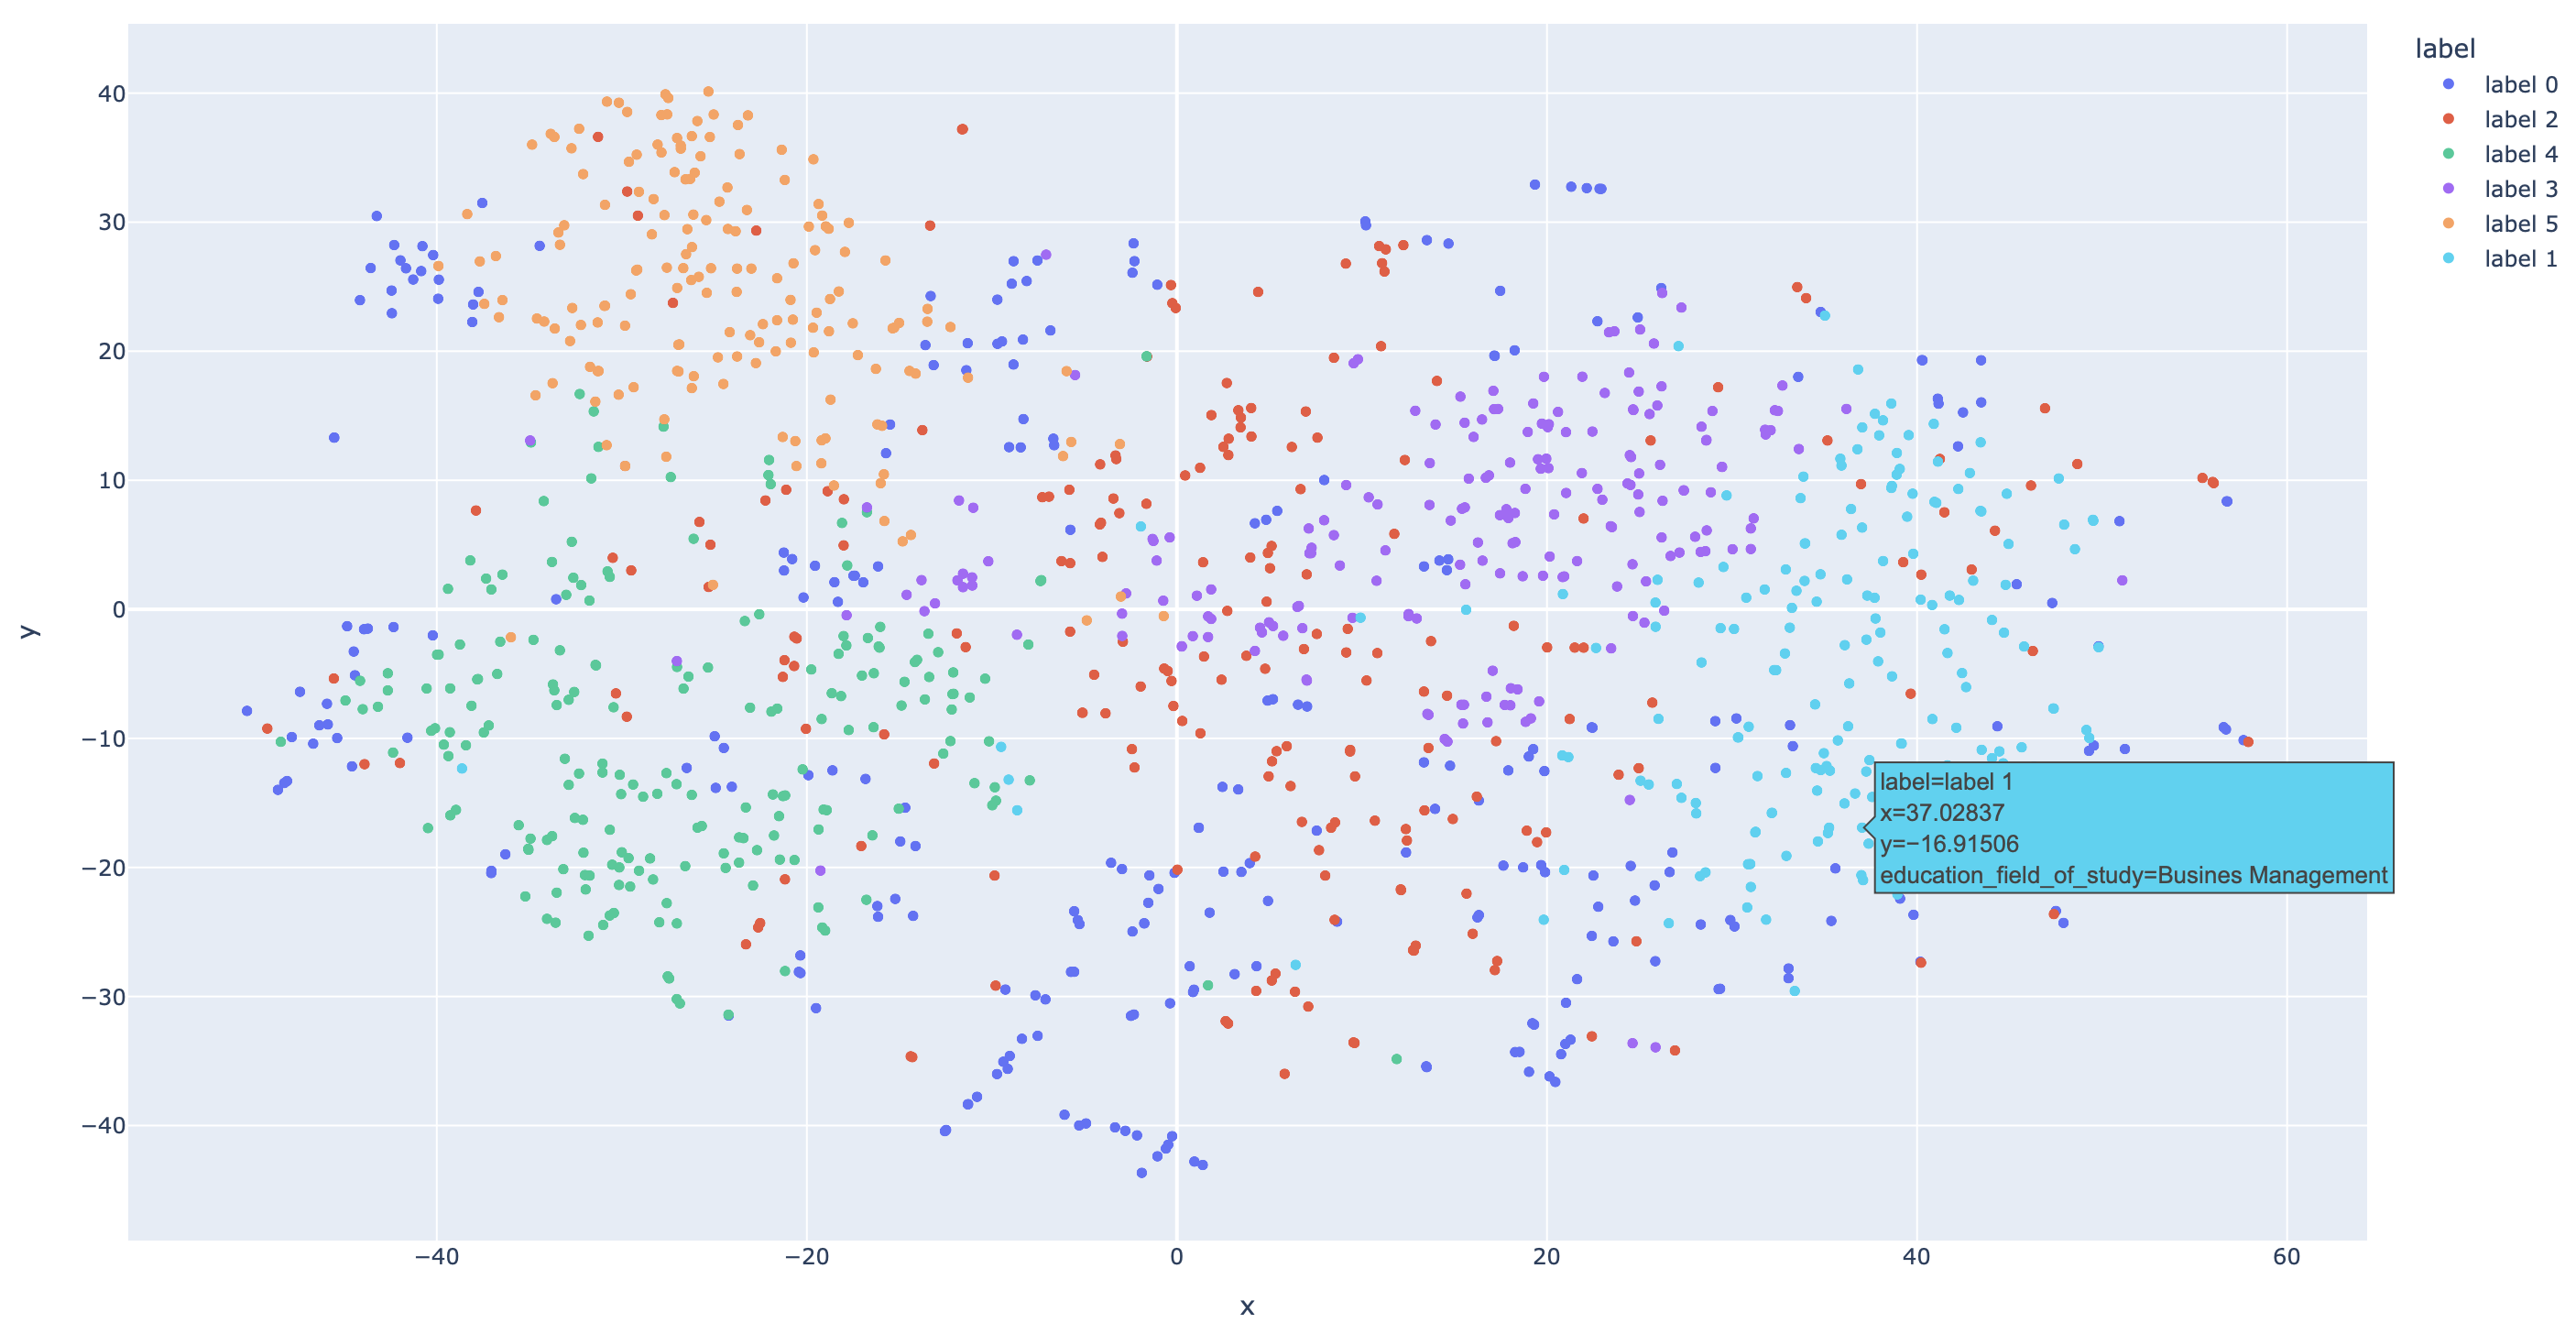
\includegraphics[width=7cm]{figures/paper/kMeans-16-03.png}
        TSNE visualization of clustered embeddings
    \end{columns}
    
\end{frame}


%\begin{frame}
%    \begin{center}
%        \Huge{Спасибо за внимание!}
%    \end{center}
%\end{frame}

\end{document}
        